\section{Memory Management}
Für ein Korrektes Speichermanagement muss der neu allozierte Speicher jewils wieder in der Laufzeit des Programmes freigegeben werden.
Die Objekte welche mit \textbf{\texttt{new}} erzeugt werden leben so lange bis sie mit \textbf{\texttt{delete}} gelöst werden.
Um speicherleaks zu verhindern braucht jedes \textbf{\texttt{new}} ein entsprechendes \textbf{\texttt{delete}}!
Speicher leaks können zu heap overflow führen.
\begin{lstlisting}[mathescape]
rational* t = new rational; 
//Speicher für t wird angelegt
rational* s = t; 
//Mehrere Zeiger auf gleiches Objekt
delete s; 
//jeder Zeiger für Freigabe möglich
int nominator = (*t).denominator(); 
//Fehler: Speicher freigegeben!
\end{lstlisting}
Korrektes Memory Management kann mit klassen implementiert werden. 
Dabei soll beachtet werden das wenn Speicher im Konstruktor alloziert wird und im Destruktor freigegeben wird nicht noch andere Pointer auf das Freigegebene Objekt zeigen.
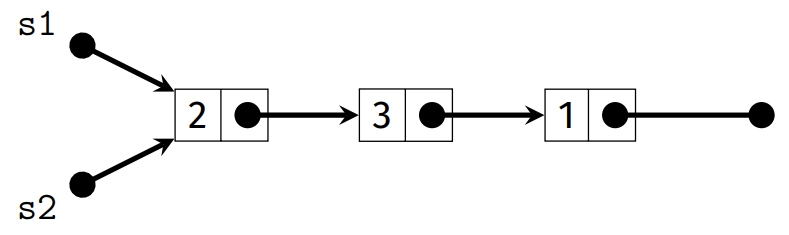
\includegraphics[width=0.24 \textwidth]{images/stack}
\begin{lstlisting}[mathescape]
stack s1;
s1.push (1);
s1.push (3);
s1.push (2);
std::cout << s1 << "\n"; // 2 3 1
stack s2 = s1;
\end{lstlisting}
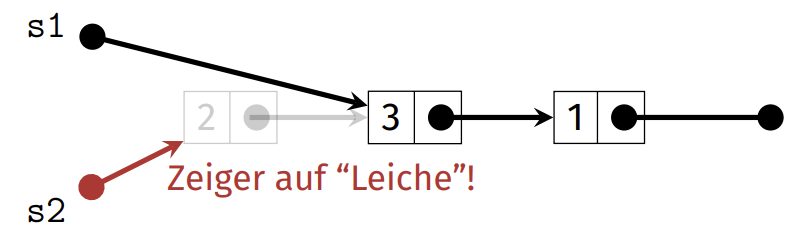
\includegraphics[width=0.24 \textwidth]{images/stack2}
\begin{lstlisting}[mathescape]
std::cout << s2 << "\n"; // 2 3 1
s1.pop ();
std::cout << s1 << "\n"; // 3 1
s2.pop (); // Programmabsturz! Pointer zeigt auf gelöschtes Objekt
\end{lstlisting}
Mögliche lösungen sind Smart-Pointer oder eine Deep-Kopie des Objektes zu erstellen.
\subsection{Smart-Pointer}
Die Idee von Smart-Pointer ist die Zeiger auf ein Objekt zu zählen und ein Objekt erst zu löschen wenn die Anzahl Pointer auf 0 fällt
\texttt{std::shared\_pointer} oder zu verhindern das mehrere Pointer auf das gleiche Objekt zeigen können \texttt{std::unique\_pointer}.
In beiden Fällen wird verhindert, dass versucht wird ein Objekt zu löschen welches schon gelöscht wurde oder noch Pointer darauf zeigen.



\subsection{Deep-Copy \& Copy Konstruktor}
Bei einer Deep-Copy oder echten Kopie eines Objektes werden alle Elemente eines Objektes Kopiert und neuem Speicher zugewiesen. 
So erhält man zwei Identische Objekte und die jeweiligen Pointer zeigen im Speicher auf zwei verschiedene Speicherabschnitte.
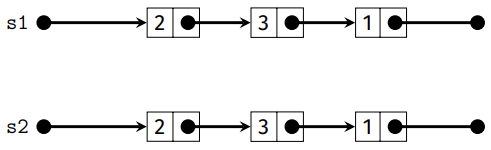
\includegraphics[width=0.24 \textwidth]{images/DeepCopy}
Dies kann mit einem Copy-Konstruktor implementiert werden. 
Der Copy-Konstruktor einer Klasse A ist erkennt man an der Deklaration \texttt{A(const A \& x);}. 
Dieser wird automatisch aufgerufen wenn Werte von Typ a initialisiert werden.
\begin{lstlisting}[mathescape]
A x = a; // a vom Typ A
A x (a);

\end{lstlisting}
Falls kein Copy-Konstruktor deklariert ist wird er automatisch erzeugt und initialisiert memberweise.
\begin{lstlisting}[mathescape]
// Coppy Konstruktor Beispiel
avec::avec(const avec& vec) : 
count(vec.count) // Init count
{	elements = new tracked[count];
	for(unsigned int i=0;i!=count;++i) 
	{
		elements[i] = vec.elements[i];
	}
}
// Destruktor Beispiel
avec::~avec() {
delete[] elements;
}
\end{lstlisting}

Das gleiche kann auch mit einer Zuweisung implementiert werden.
Dazu wird der \texttt{=} Operator überladen.
\begin{lstlisting}[mathescape]
avec& avec::operator=(const avec& t) 
{
	if (elements != t.elements) 
	// keine Selbstzuweisung
	{
		avec copy(t); // Kopierkonstruktor
		std::swap(copy.elements, elements);  
		// copy hat nun den Müll!
		std::swap(copy.count, count); 
		//copy wird aufgeräumt $\rightarrow$ Dekonstruktion
	}
	return(*this); // Rueckgabe als L-Wert (Konvention)
}
\end{lstlisting}
Ein gutes Memory Management kann im Header file erkannt werden wenn alle Fälle des Kopierens einer Klasse abgedeckt sind:
\begin{itemize}
	\item Konstruktoren
	\item Destruktoren
	\item Copy-Construktor
	\item Zuweisungsoperator
\end{itemize}
Daraus ergibt sich die Dreierregel: definiert eine Klasse eines der letzen drei, so muss sie auch die anderen zwei definieren!

\begin{lstlisting}[mathescape]
avec(unsigned int size); //Constructor
avec(const avec& vec); //Copy-Constructor
avec& operator=(const avec& vec);
//assignment operator
~avec(); //Destructor
\end{lstlisting}













